% Generated on 2023-07-18 11:23:23 by gEcon ver. 1.2.1 (2023-01-18)
% http://gecon.r-forge.r-project.org/

% Model name: RW

\section{Steady-state values}


\begin{tabular}{c|c|}
  & Steady-state value\\
\hline
$i$ & 1 \\
$\lambda^{\mathrm{RW}^{\mathrm{1}}}$ & 0 \\
$\lambda^{\mathrm{RW}^{\mathrm{2}}}$ & 0 \\
$\pi$ & 0 \\
${r\!n}$ & 1 \\
$y$ & 0 \\
$U$ & 0 \\
\hline
\end{tabular}


\section{The solution of the 1st order perturbation}

\subsection*{Matrix $P$}

$$\bordermatrix{
~ & i_{t-1} & \pi_{t-1} & {r\!n}_{t-1} & y_{t-1} \cr
i_{t} & -1.9422 & 5.8224 & 2.8922 & -3.3774 \cr
\pi_{t} & 0 & 1.0101 & 0 & -0.249 \cr
{r\!n}_{t} & 0 & 0 & 0.95 & 0 \cr
y_{t} & 1 & -1.0101 & -1 & 1.249 \cr
}$$

\subsection*{Matrix $Q$}

$$\bordermatrix{
~ & \epsilon^{\mathrm{Z}} \cr
i & 1 \cr
\pi & 0 \cr
{r\!n} & 1 \cr
y & 0 \cr
}$$

\subsection*{Matrix $R$}

$$\bordermatrix{
~ & i_{t-1} & \pi_{t-1} & {r\!n}_{t-1} & y_{t-1} \cr
\lambda^{\mathrm{RW}^{\mathrm{1}}}_{t} & -0.5005 & 3.4065 & 0.5005 & -1.3402 \cr
\lambda^{\mathrm{RW}^{\mathrm{2}}}_{t} & 0.1309 & -0.5005 & -0.1309 & 0.2543 \cr
U_{t} & 0 & 0 & 0 & 0 \cr
}$$

\subsection*{Matrix $S$}

$$\bordermatrix{
~ & \epsilon^{\mathrm{Z}} \cr
\lambda^{\mathrm{RW}^{\mathrm{1}}} & 0 \cr
\lambda^{\mathrm{RW}^{\mathrm{2}}} & 0 \cr
U & 0 \cr
}$$


\section{Model statistics}

\subsection{Basic statistics}

\begin{tabular}{c|c|c|c|c|}
  & Steady-state value & Std. dev. & Variance & Loglin\\
\hline
$i$ & 1 & 0.1303 & 0.017 & Y    \\
$\lambda^{\mathrm{RW}^{\mathrm{1}}}$ & 0 & 0 & 0 & N    \\
$\lambda^{\mathrm{RW}^{\mathrm{2}}}$ & 0 & 0 & 0 & N    \\
$\pi$ & 0 & 0 & 0 & N    \\
${r\!n}$ & 1 & 0.1303 & 0.017 & Y    \\
$y$ & 0 & 0 & 0 & N    \\
$U$ & 0 & 0 & 0 & N    \\
\hline
\end{tabular}


\subsection{Correlation matrix}

\begin{tabular}{c|cc|}
  & $i$ & ${r\!n}$\\
\hline
$i$ & 1 & 1 \\
${r\!n}$ &  & 1 \\
\hline
\end{tabular}


\subsection{Cross correlations with the reference variable ($i$)}

\begin{tabular}{c|c|c|c|c|c|c|c|c|c|c|c|c|}
  & $\sigma[\cdot]$ rel. to $\sigma[i]$ & $i_{t-5}$ & $i_{t-4}$ & $i_{t-3}$ & $i_{t-2}$ & $i_{t-1}$ & $i_{t}$ & $i_{t+1}$ & $i_{t+2}$ & $i_{t+3}$ & $i_{t+4}$ & $i_{t+5}$\\
\hline
$i_{t}$ & 1 & -0.016 & 0.11 & 0.271 & 0.471 & 0.713 & 1 & 0.713 & 0.471 & 0.271 & 0.11 & -0.016 \\
${r\!n}_{t}$ & 1 & -0.016 & 0.11 & 0.271 & 0.471 & 0.713 & 1 & 0.713 & 0.471 & 0.271 & 0.11 & -0.016 \\
\hline
\end{tabular}


\subsection{Autocorrelations}

\begin{tabular}{c|ccccc|}
  & Lag 1 & Lag 2 & Lag 3 & Lag 4 & Lag 5\\
\hline
$i$ & 0.713 & 0.471 & 0.271 & 0.11 & -0.016 \\
${r\!n}$ & 0.713 & 0.471 & 0.271 & 0.11 & -0.016 \\
\hline
\end{tabular}



\pagebreak

\section{Impulse response functions}

\begin{figure}[h]
\centering
\begin{minipage}{0.5\textwidth}
\vspace*{-3em}
\centering
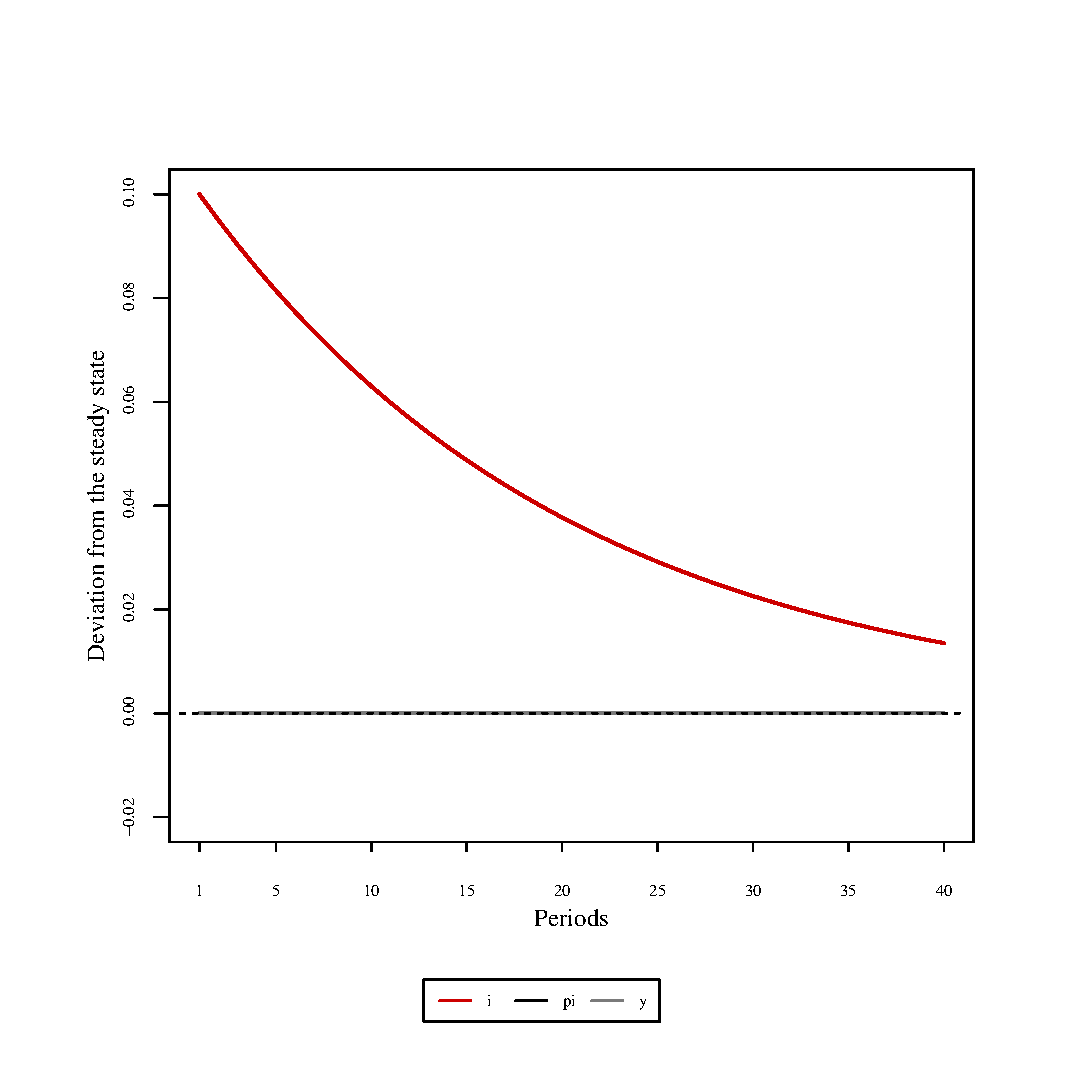
\includegraphics[width=0.99\textwidth, scale=0.55]{plots/plot_11.eps}
\caption{Impulse responses ($i, \pi, y$) to $\epsilon^{\mathrm{Z}}$ shock}
\end{minipage}
\end{figure}
